\section{RASD}

	\subsection{Goals}
		\begin{frame}{Goals}
			\vspace{-17pt}
			\begin{enumerate}[label=\textbf{G\arabic*}]\small
				\item \label{goal:notification} Users should be able to notify authorities when traffic violations occur, in particular parking violations.
				\item \label{goal:mining} Users and authorities should be able to mine the information stored by SafeStreets, with different levels of visibility.
				\begin{enumerate}[label=\textbf{G2\Alph*}]
					\item \label{goal:miningA} Users and authorities should be able to know where the highest number of violations occur.
					\item \label{goal:miningB} Users and authorities should be able to know what types of vehicle make the most violations.
					\item \label{goal:miningC} Authorities should be able to consult every violation report sent by users.
				\end{enumerate}
				\item \label{goal:safety} Users should be able to know which streets are safe and which ones are not.
				\item \label{goal:intervention} Users and authorities should be able to know the possible interventions that could be done in a city.
			\end{enumerate}
		\end{frame}

	\subsection{Boundaries of the system}
		\begin{frame}{System Interfaces}
			We want now to define the boundaries of our system first with the external interfaces it has to interact with, second with the \emph{World And Machine} that helps to highlight the phenomena.
			
			\begin{figure}[h!]
				\centering
				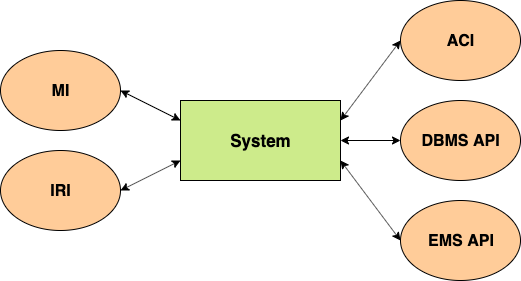
\includegraphics[scale=0.48]{rasd/externalInterfaces.png}
			\end{figure}
		\end{frame}
		
		\begin{frame}{The World and the Machine}
			\vspace{-24pt}
			\begin{figure}[hbtp]
				\centering
				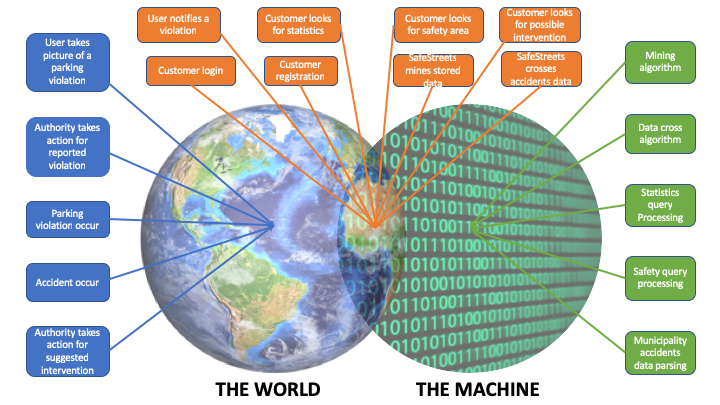
\includegraphics[scale=0.44]{rasd/WorldAndMachine}
			\end{figure}
		\end{frame}
	
	\subsection{Meaningful Use-Cases}
		\begin{frame}{User Notification}
				\begin{minipage}{0.4\textwidth}
					\begin{flushleft}
						\begin{figure}[ht]
							\centering
							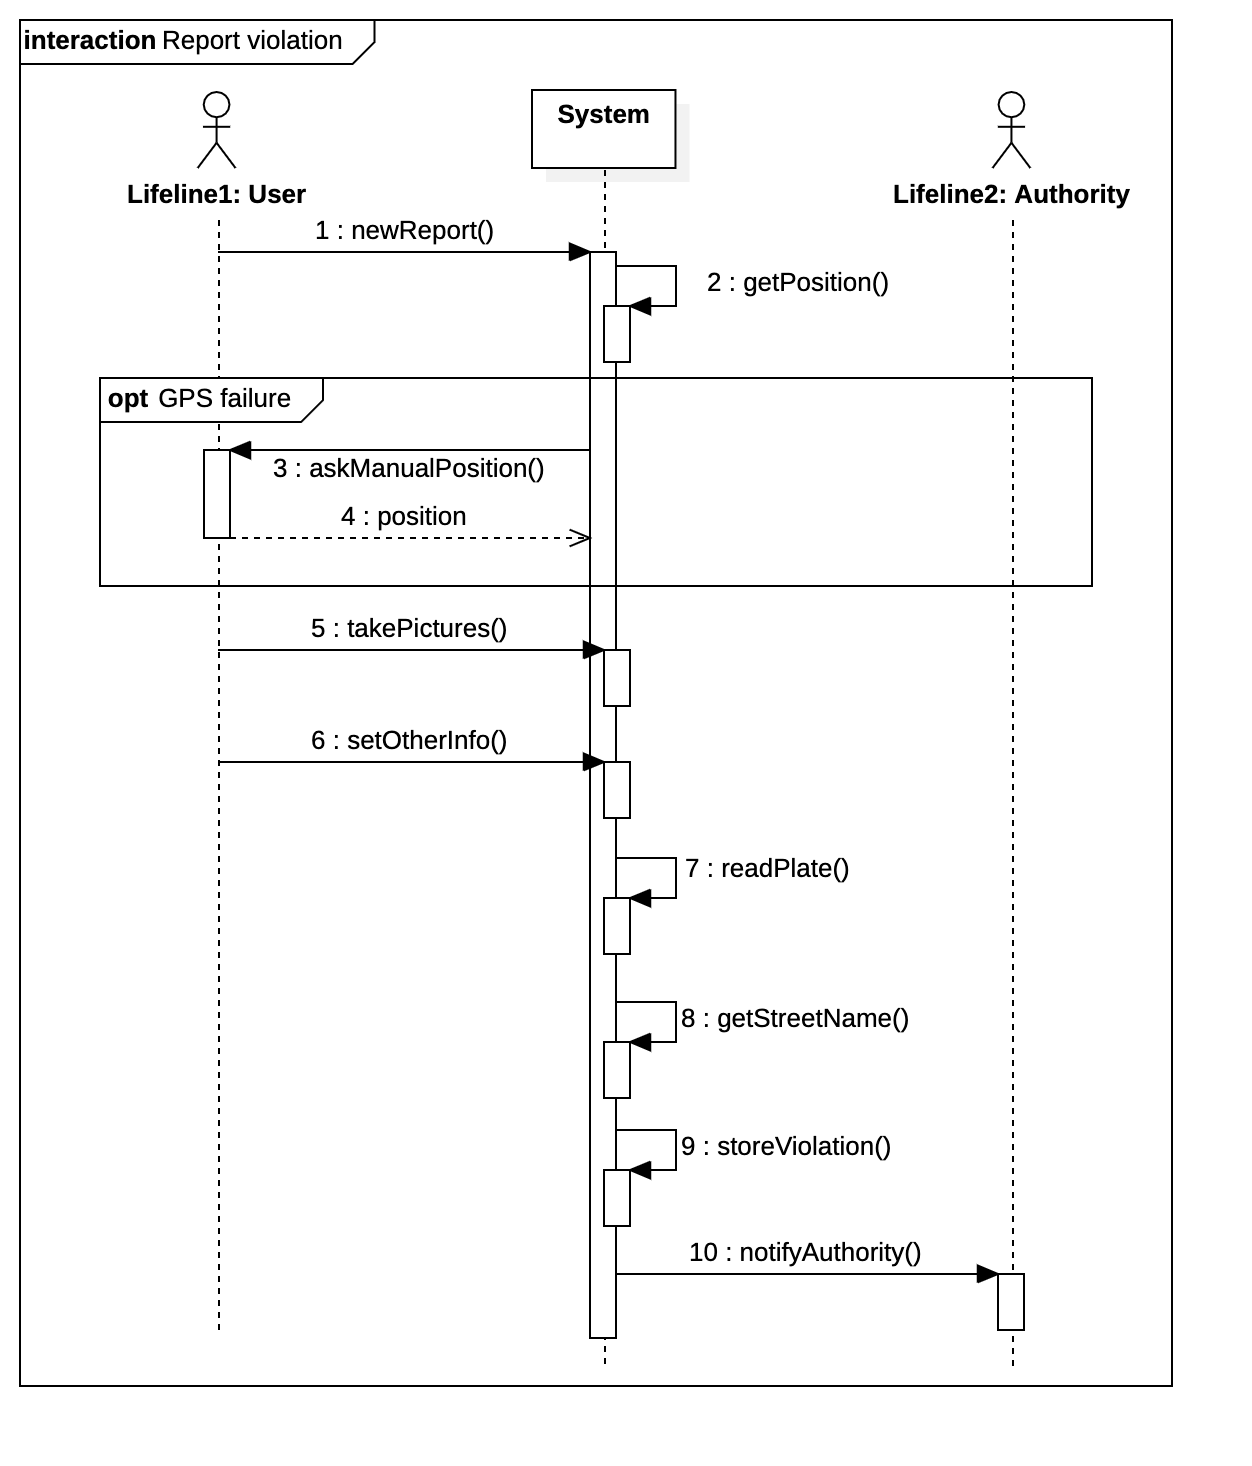
\includegraphics[scale=0.14]{rasd/reportViolation}
						\end{figure}
					\end{flushleft}
				\end{minipage}\hfill
				~
				\begin{minipage}{0.43\textwidth}\small
					Qua ci potrebbe stare una descrizione con elenco:
					\begin{itemize}
						\item 
						\item 
						\item 
					\end{itemize}
				\end{minipage}
		\end{frame}
	
		\begin{frame}{Unsafe Streets Functionality}
			\begin{figure}[hbtp]
				\centering
				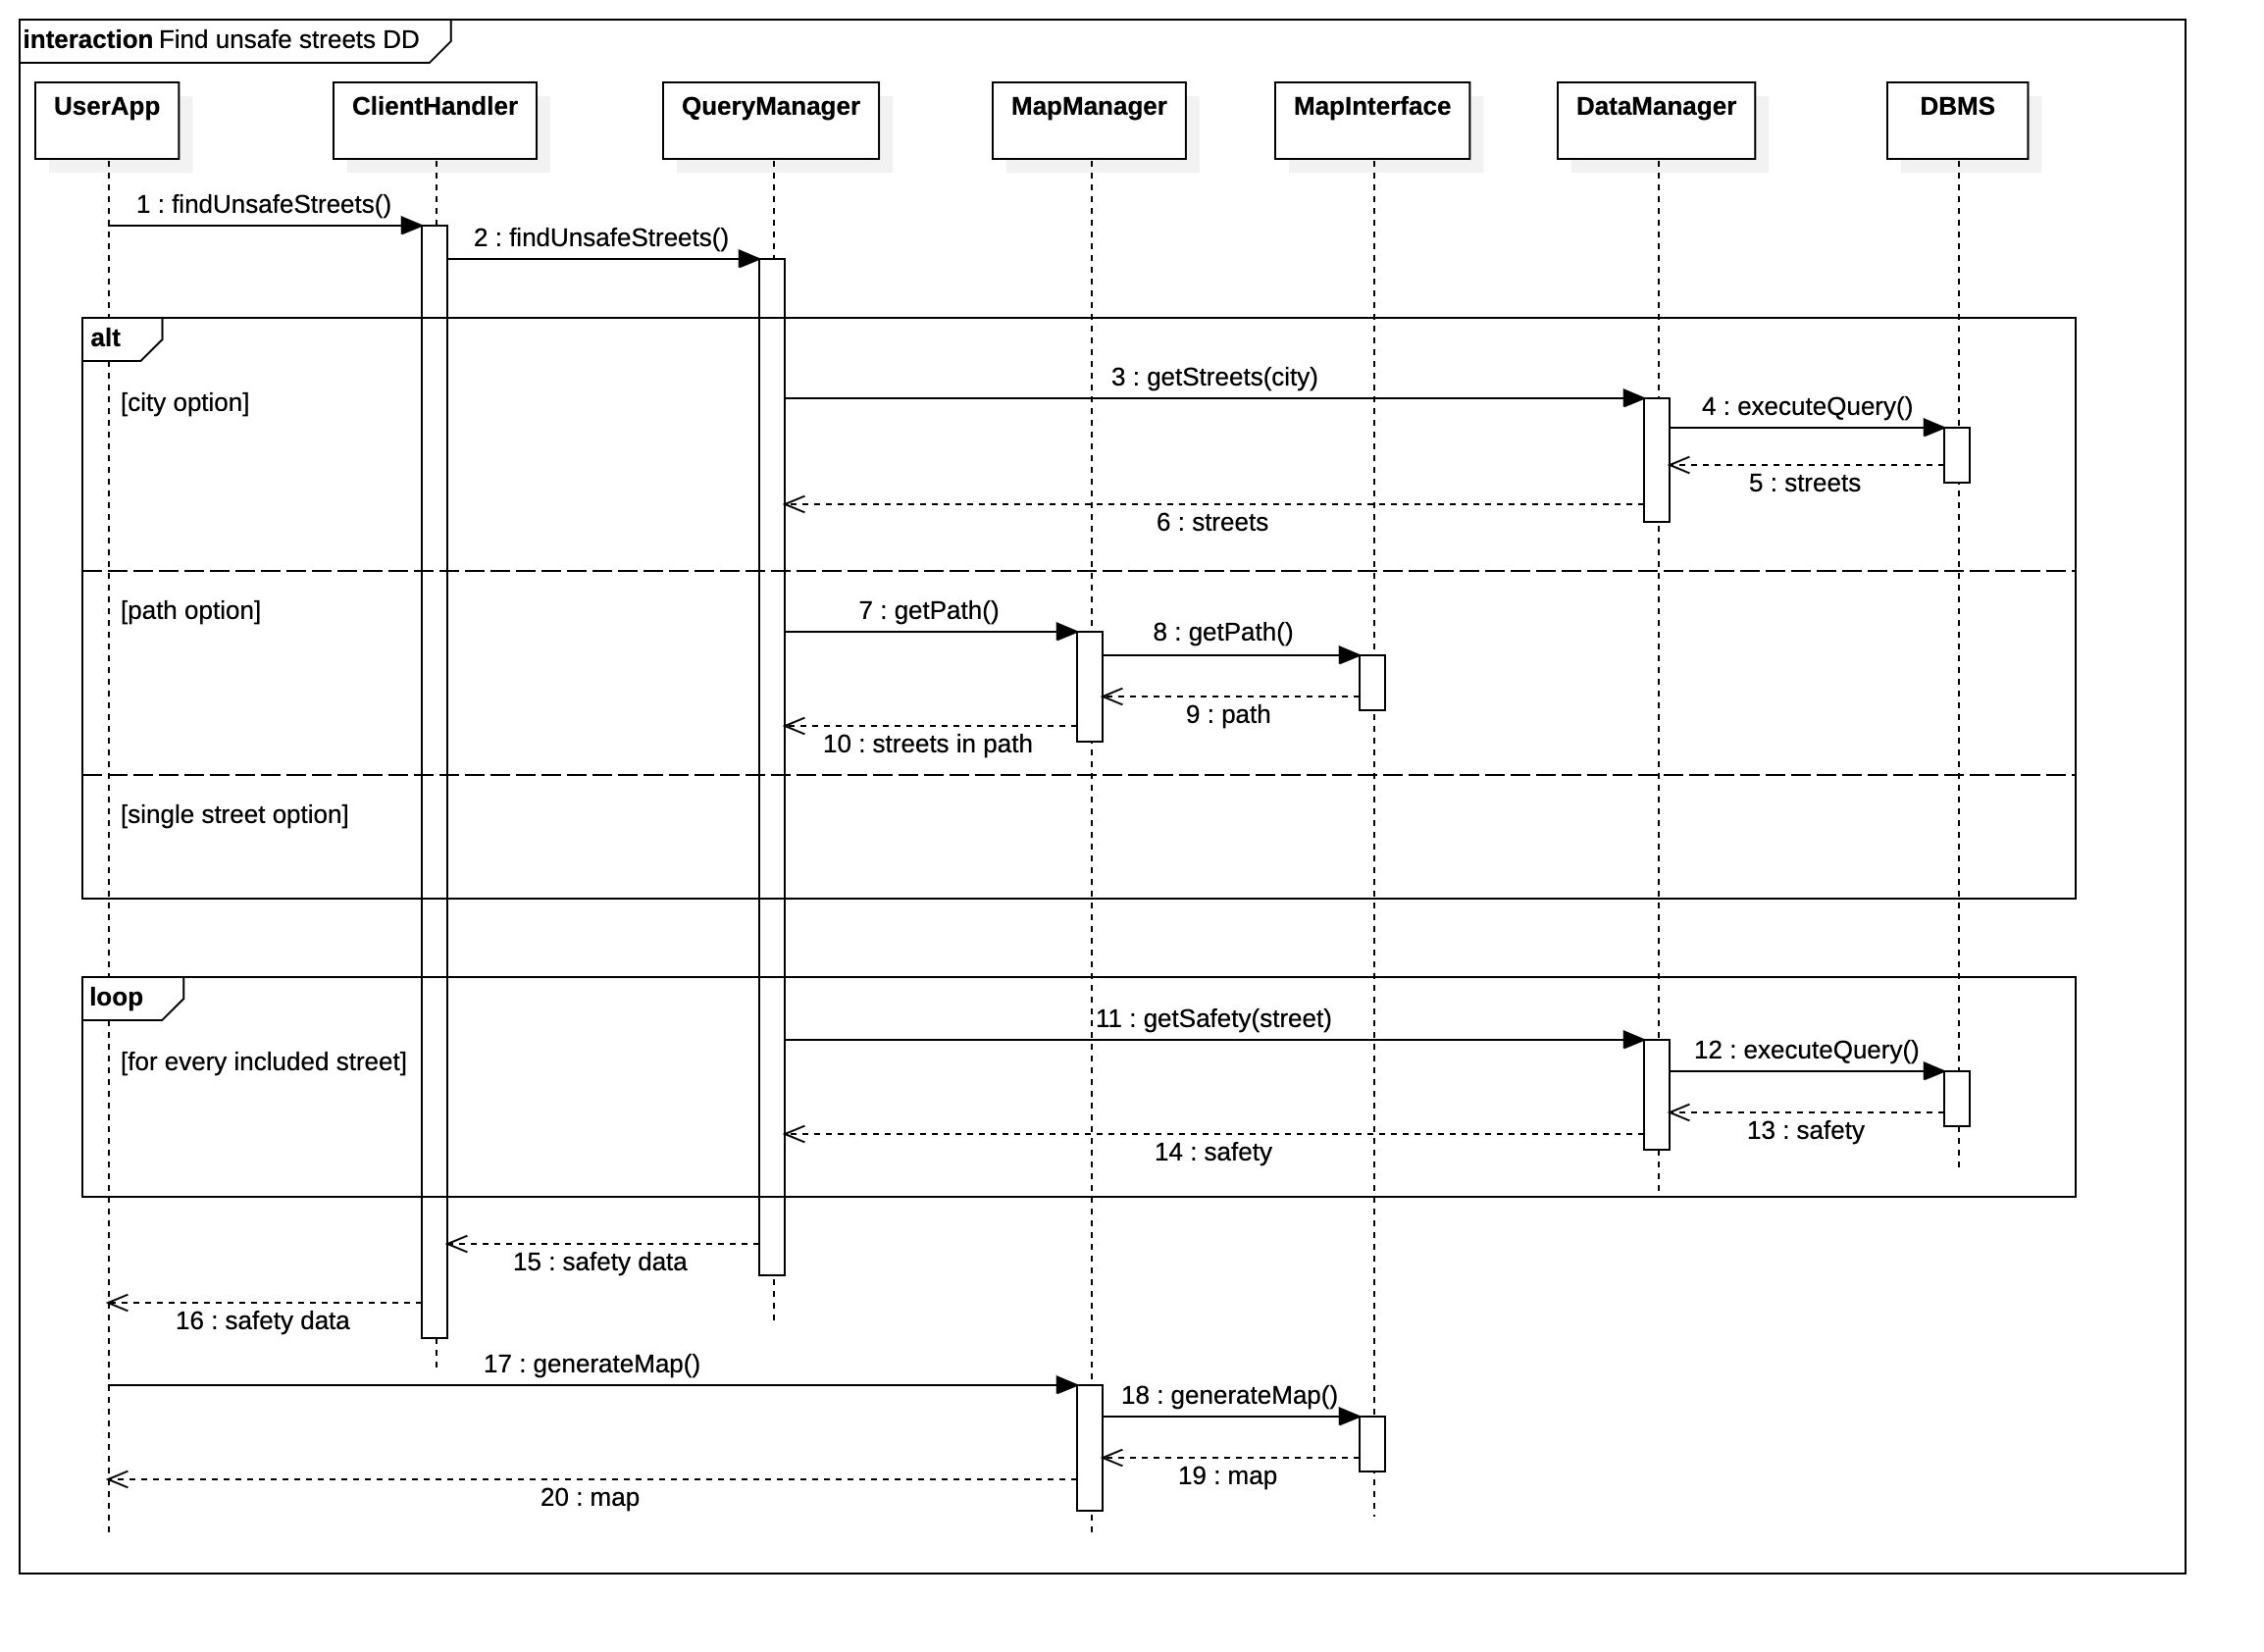
\includegraphics[scale=0.14]{rasd/unsafeStreets}
			\end{figure}
		\end{frame}
	
		\begin{frame}{Check and Find Reports}
			\begin{minipage}{0.4\textwidth}
				\begin{figure}
					\centering
					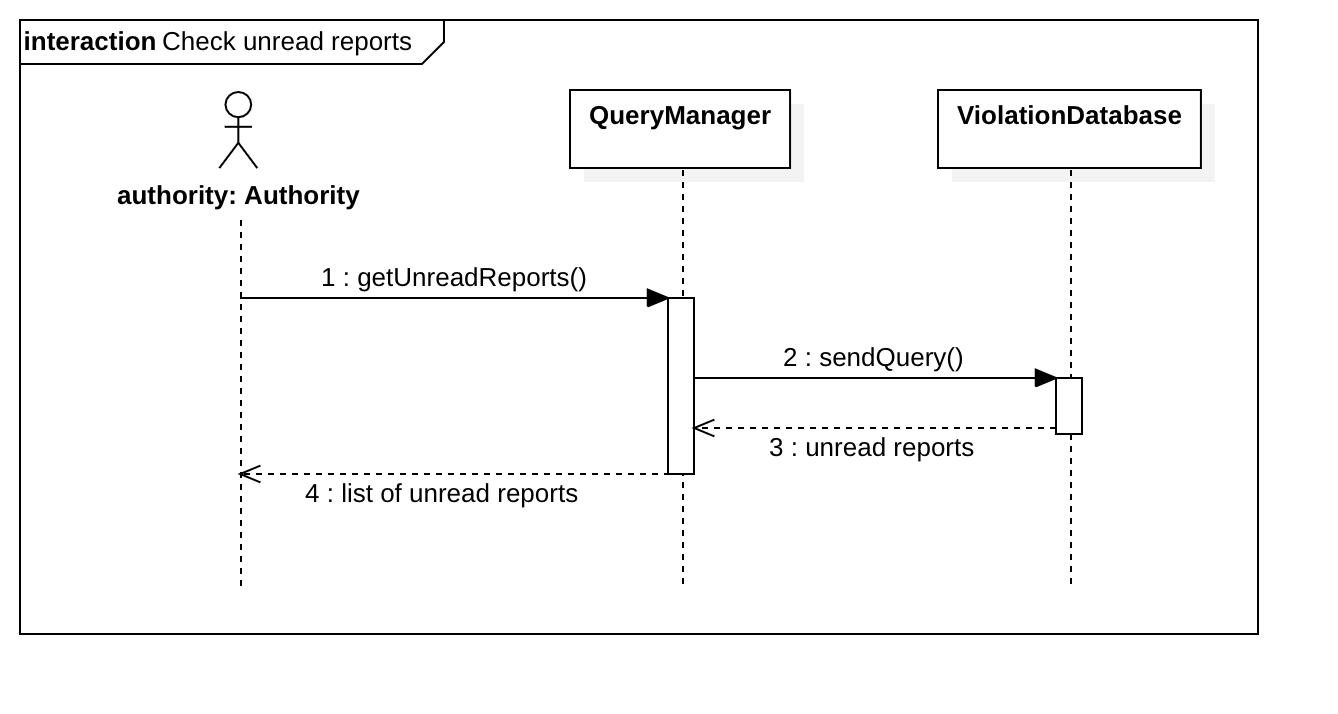
\includegraphics[scale=0.15]{rasd/unreadReports}
				\end{figure}
			\end{minipage}\hfill
			~
			\begin{minipage}{0.4\textwidth}
				\begin{figure}
					\centering
					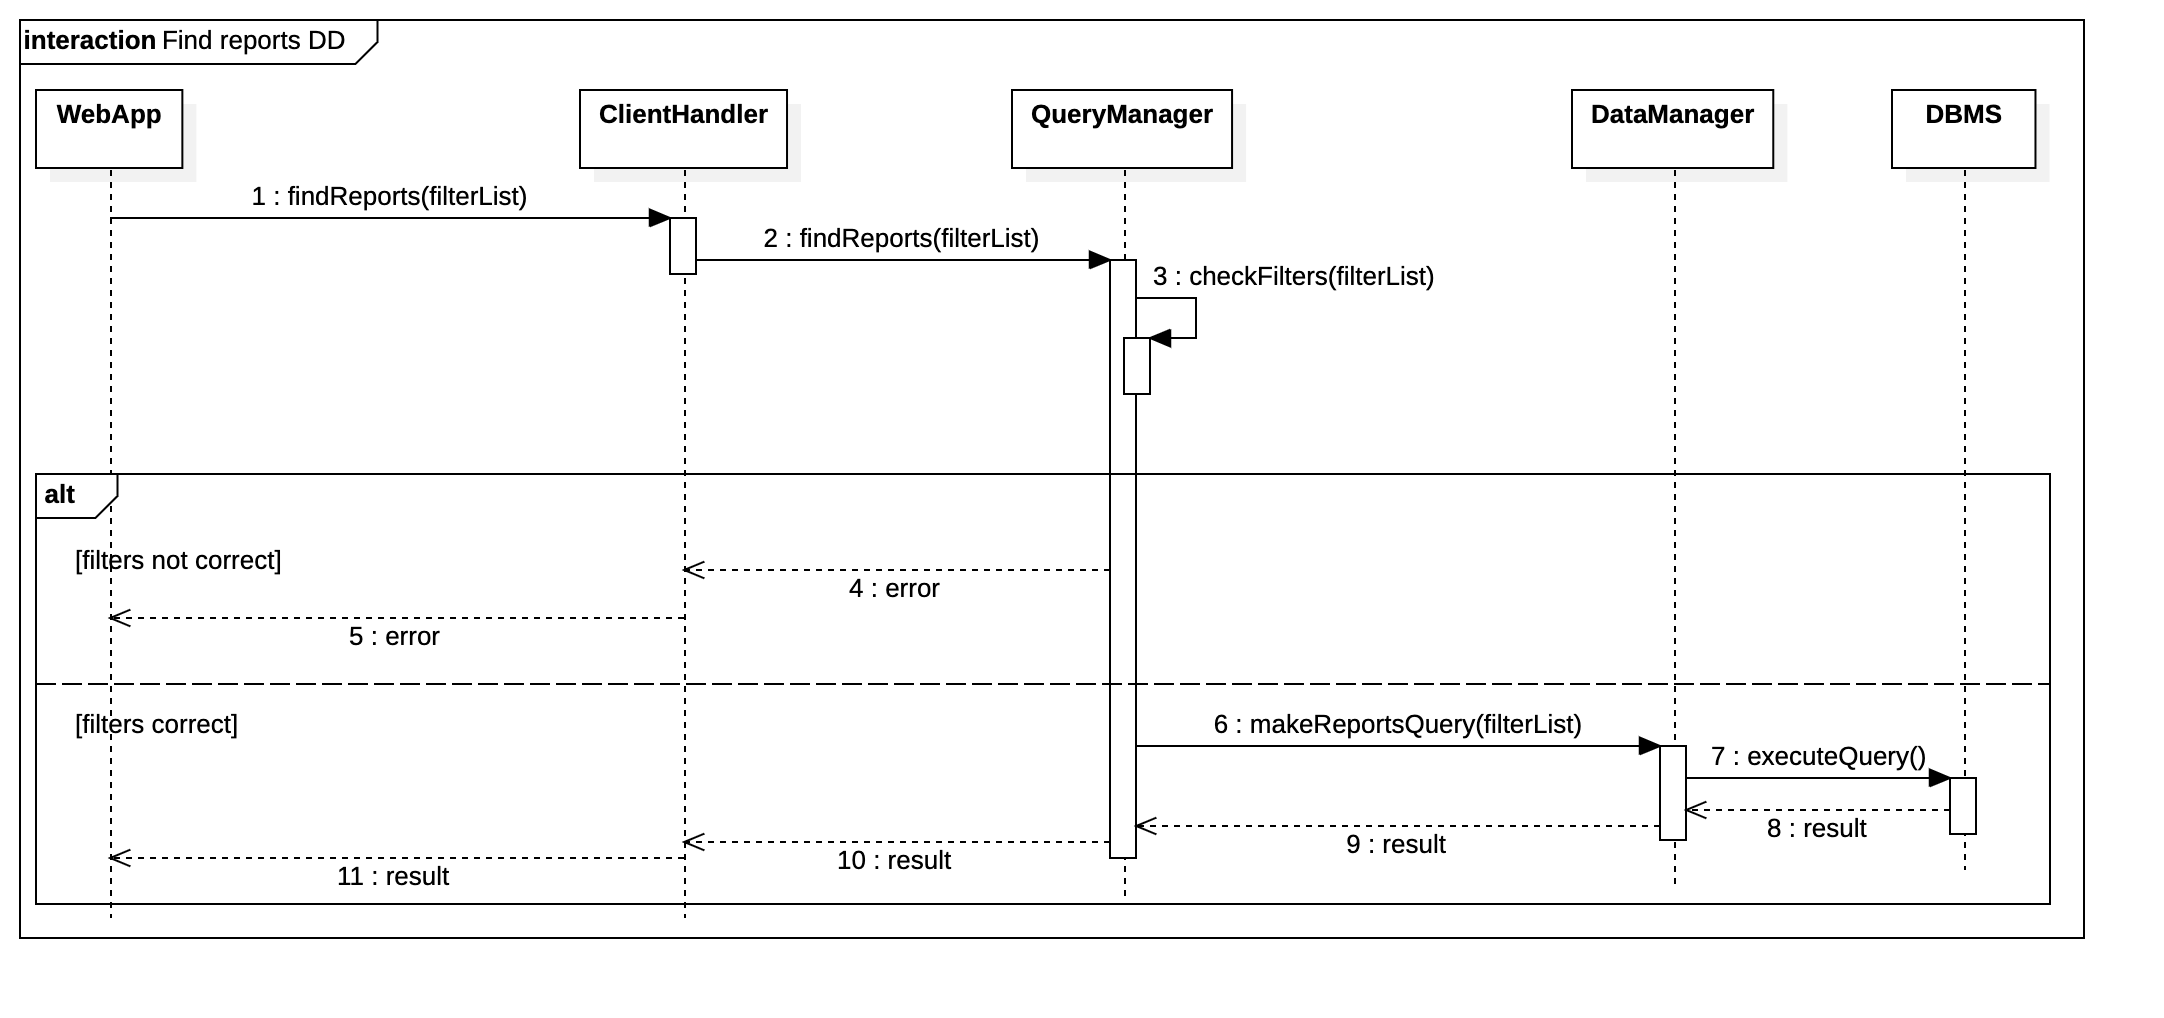
\includegraphics[scale=0.12]{rasd/findReports}
				\end{figure}
			\end{minipage}
			
		\end{frame}
